\usetikzlibrary{arrows,positioning}
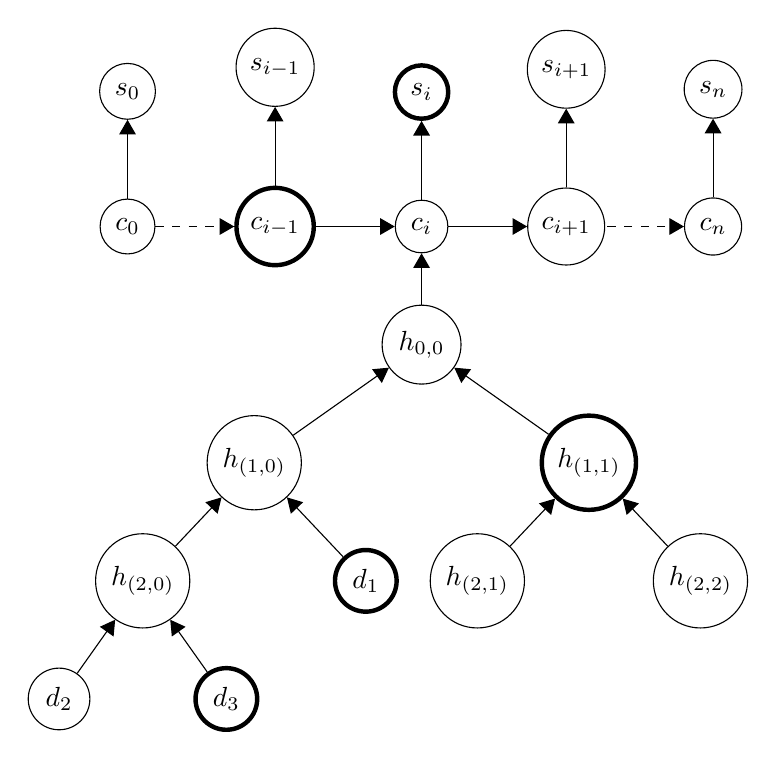
\begin{tikzpicture}[level/.style={sibling distance=85mm/#1}, 
                                    every node/.style={circle,draw},
                                    every path/.style={<-,>=triangle 60}]
\node (ci) {$c_i$}
child {node (h00){$h_{0,0}$}
  child {node (h10) {$h_{(1,0)}$}
    child {node (h20) {$h_{(2,0)}$}
      child {node (d2) {$d_2$}}
      child {node [ultra thick] (d3) {$d_3$}}
    }
    child {node [ultra thick] (h20) {$d_1$}}
  }
  child {node [ultra thick] (h11) {$h_{(1,1)}$}
    child {node (h21) {$h_{(2,1)}$}}
    child {node (h22) {$h_{(2,2)}$}}
  }
};

\node[above=of ci,ultra thick] (sn) {$s_i$} edge(ci);

\node[left=of ci,ultra thick] (ciminus) {$c_{i-1}$} edge[->] (ci);
\node[right=of ci] (ciplus) {$c_{i+1}$} edge[<-] (ci);

\node[above=of ciminus] (siminus) {$s_{i-1}$} edge (ciminus);
\node[above=of ciplus] (siplus) {$s_{i+1}$} edge (ciplus);

\node[left=of ciminus] (c0) {$c_0$} edge[->,dashed] (ciminus);
\node[right=of ciplus] (cn) {$c_n$} edge[<-,dashed] (ciplus);

\node[above=of c0] (s0) {$s_0$} edge (c0);
\node[above=of cn] (sn) {$s_n$} edge (cn);

\end{tikzpicture}